\documentclass[12pt,a4paper]{article}
\usepackage{physics}
\usepackage{amssymb}
\usepackage{subcaption}
\usepackage{colortbl}
\newcommand{\activity}{Activity 8 -- Color Difference}
\input{spp.dat}

%  Editorial staff will uncomment the next line
% \providecommand{\artnum}[0]{XX-XX}
% \renewcommand{\articlenum}[0]{SPP-\the\year-\artnum-}

\begin{document}

\title{\TitleFont \activity}
\author[ ]{\textbf{Kenneth V. Domingo} \\
2015--03116 \\
App Physics 187, 1\textsuperscript{st} Semester, A.Y. 2019--20}
\affil[ ]{\corremail{kvdomingo@up.edu.ph} }

\maketitle
\thispagestyle{titlestyle}

\section*{Results and Discussion}
\setcounter{section}{1}

For this activity, the values for CIE 1964 standard observer, standard illuminant D65, illuminant D55, and their respective white point tristimulus values were obtained from \cite{cie64}. The reflectances of the Macbeth patches were obtained from \citep{soriano}. Interpolation was performed for all the data to ensure that they are all aligned and of the same length. The tristimulus values for each patch under an illuminant were obtained by

\begin{equation}\label{eq:tristimulus}
	T = \int M(\lambda) R(\lambda) \bar{t}(\lambda) \dd{\lambda}
\end{equation}

\noindent where $M$ is the spectral power distribution of the illuminant, $R$ is the reflectance of a patch, $\bar{t}$ is a standard observer, and $T$ is a tristimulus value. From here, conversion to $La^\star b^\star$ was performed using

\begin{equation}\label{eq:XYZ2Lab}
\begin{aligned} 
	L &= 116 f\qty(\frac{Y}{Y_n}) - 16 \\
	a^\star &= 500\qty[f\qty(\frac{X}{X_n}) - f\qty(\frac{Y}{Y_n})]  \\
	b^\star &= 200\qty[f\qty(\frac{Y}{Y_n}) - f\qty(\frac{Z}{Z_n})]
\end{aligned}
\end{equation}

\noindent where

\begin{align*}
	f(t) &=
	\begin{cases}
		\sqrt[3]{t} & t > \delta^3 \\
		\frac{t}{3\delta^2} + \frac{4}{29} & \textrm{otherwise}
	\end{cases} \\
	\delta &= \frac{6}{29}
\end{align*}

\noindent where $X_n, Y_n, Z_n$ are the white point tristimulus values. Conversion to $LC^\star h$ was performed using

\begin{equation}\label{eq:LabtoLCh}
\begin{aligned}
	C^\star &= \sqrt{a^{\star 2} + b^{\star 2}} \\
	h &= \arctan{\frac{b^\star}{a^\star}}
\end{aligned}
\end{equation}

\noindent The color differences in $La^\star b^\star$ and $LC^\star h$ are respectively calculated by

\begin{align}
	\Delta E(a^\star, b^\star) &= \sqrt{\qty(\Delta L)^2 + \qty(\Delta a^\star)^2 + \qty(\Delta b^\star)^2} \label{eq:LabDE} \\
	\Delta E(C^\star, h) &= \sqrt{\qty(\Delta L)^2 + \qty(\Delta C^\star)^2 + \qty(\Delta h)^2} \label{eq:LChDE}
\end{align}

\noindent The results of applying \eqref{eq:LabDE}--\eqref{eq:LChDE} on each Macbeth patch is shown in Table \ref{tab:color-diff}. Figure \ref{fig:macbeth} shows the reference Macbeth chart.

\begin{table}[!htb]
	\centering
	\caption{Color difference values for the Macbeth patches under D65 and D55 illumination.}
	\begin{tabular}{||r|r|r||}
		\hline
		Patch & $La^\star b^\star \Delta E$ & $LC^\star h \Delta E$ \\ \hline \hline
		1  & 3.14 & 3.10 \\
		2  & 4.43 & 4.16 \\
		3  & 2.96 & 2.67 \\
		4  & 2.40 & 2.23 \\
		5  & 2.77 & 2.65 \\
		6  & 3.11 & 2.92 \\
		7  & 6.10 & 6.04 \\
		8  & 3.76 & 2.51 \\
		9  & 5.10 & 5.04 \\
		10 & 1.80 & 1.74 \\
		11 & 4.22 & 3.60 \\
		12 & 6.12 & 5.82 \\
		13 & 4.38 & 2.49 \\
		14 & 2.58 & 2.56 \\
		15 & 5.76 & 5.73 \\
		16 & 6.29 & 5.39 \\
		17 & 3.79 & 3.54 \\
		18 & 4.12 & 4.08 \\
		19 & 4.18 & 4.14 \\
		20 & 3.62 & 4.43 \\
		21 & 3.07 & 3.92 \\
		22 & 2.54 & 3.51 \\
		23 & 1.94 & 1.98 \\
		24 & 1.37 & 1.38 \\ \hline
	\end{tabular}
	\label{tab:color-diff}
\end{table}

\begin{figure}
	\centering
	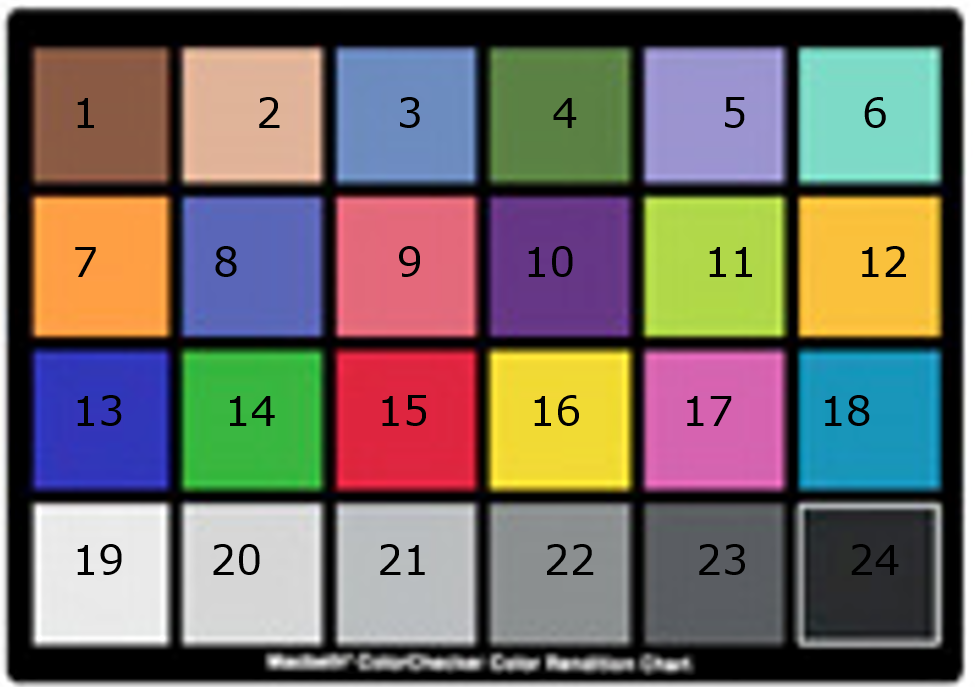
\includegraphics[width=0.7\textwidth]{macbeth.png}
	\caption{Reference Macbeth color chart.}
	\label{fig:macbeth}
\end{figure}


\bibliographystyle{spp-bst}
\bibliography{biblio}

\end{document}